\documentclass[conference,a4paper,10pt]{IEEEtran}

% --- packages ---------------------------------------------------------------
\usepackage[utf8]{inputenc}
\usepackage[T1]{fontenc}
\usepackage{lmodern}
\usepackage{graphicx}
\usepackage{booktabs}
\usepackage{tabularx}
\usepackage{array}
\usepackage{xcolor}
\usepackage{tikz}
\usepackage{caption}
\usepackage{subcaption}
\usepackage{hyperref}
\usepackage{url}
\usepackage{microtype}
\usepackage{cite}

\graphicspath{{figures/}}

% Smart placeholder: if the screenshot exists in figures/, embed it;
% otherwise render a labelled box explaining what to capture.
% Usage: \screenshot{filename.png}{0.95\linewidth}{Description text}
\newcommand{\screenshot}[3]{%
  \IfFileExists{figures/#1}{%
    \includegraphics[width=#2]{#1}%
  }{%
    \fbox{\parbox[c][3.5cm][c]{#2}{\centering\small\textit{Screenshot placeholder}\\\textbf{File:} \texttt{#1}\\\small #3}}%
  }%
}

\hypersetup{
  colorlinks=true,
  linkcolor=black,
  citecolor=black,
  urlcolor=blue,
  pdftitle={End-to-End MLOps for Customer Churn Prediction},
  pdfauthor={Dan Waititu}
}

% --- title ------------------------------------------------------------------
\title{End-to-End MLOps for Customer Churn Prediction:\\
       From Training to Drift-Aware Monitoring with a Reproducible
       Container Stack}

\author{\IEEEauthorblockN{Dan Waititu}\\
\IEEEauthorblockA{Lucerne University of Applied Sciences and Arts (HSLU)\\
MSc Module: Artificial Intelligence\\
\textit{danwwaititu@gmail.com}}}

% ---------------------------------------------------------------------------
\begin{document}
\maketitle

\begin{abstract}
This report describes the design, implementation and operation of an
end-to-end machine-learning operations (MLOps) pipeline for binary
customer-churn prediction on the well-known IBM Telco dataset. The
system pairs a dual-model gradient-boosting ensemble
(LightGBM~\cite{ke2017lightgbm} and XGBoost~\cite{chen2016xgboost}) with
Bayesian hyper-parameter optimisation via Optuna~\cite{akiba2019optuna},
five-fold stratified cross-validation, and an MLflow~\cite{mlflow_docs}
registry-backed promotion workflow. Predictions are served through a
FastAPI~\cite{fastapi_docs} web service inside a Docker
Compose~\cite{docker_compose} topology that includes Postgres, Grafana
and a replay-based monitoring worker which writes
Evidently~\cite{evidently_docs} drift and quality metrics to a relational
store visualised by an eight-panel Grafana dashboard. A multi-workflow
GitHub Actions~\cite{gha_docs} pipeline enforces linting, testing,
coverage, container builds with SLSA provenance~\cite{slsa_v1} and
weekly secret scanning. The artefact closes the MLOps loop end to end on
a single developer workstation and is reproducible by a single
\textsc{docker~compose~up} invocation. The contribution of this work is
not a new modelling result but a documented, integrated reference
implementation of the operational practices distilled by Sculley
\emph{et~al.}~\cite{sculley2015hidden} and Paleyes
\emph{et~al.}~\cite{paleyes2022deploy}.
\end{abstract}

\begin{IEEEkeywords}
MLOps, customer churn, gradient boosting, model registry, drift
detection, continuous integration, reproducibility.
\end{IEEEkeywords}

% ===========================================================================
\section{Introduction}\label{sec:intro}

Customer churn---the rate at which existing customers terminate their
relationship with a service provider---is a recurring concern in
subscription industries because acquiring a new customer is materially
more expensive than retaining an existing one~\cite{verbeke2012churn}.
Predictive churn modelling allows targeted retention interventions, but
the value of such a model is realised only once it is deployed,
monitored and re-trained inside an organisational workflow.

A long line of empirical work has documented that the modelling code is
the smallest part of a production ML system; the much larger surface
area consists of data plumbing, configuration management, monitoring
infrastructure, serving infrastructure and governance
controls~\cite{sculley2015hidden,paleyes2022deploy}. The discipline of
MLOps emerged to address this imbalance by transferring established
software-engineering practices---continuous integration, infrastructure
as code, observability, version control of artefacts---into the ML
lifecycle.

This report documents an end-to-end MLOps reference implementation
built for the HSLU Artificial Intelligence module. The system targets
the IBM Telco customer-churn dataset and integrates ten open-source
tools into a single \textsc{docker~compose} stack. The deliverables are:
\begin{enumerate}
  \item a training pipeline that performs Bayesian hyper-parameter
        optimisation followed by stratified cross-validation of a dual
        LightGBM/XGBoost ensemble, logging every artefact to MLflow;
  \item a FastAPI serving layer that loads the currently aliased
        \textsc{champion} model from the MLflow registry at start-up and
        applies the same preprocessing as training;
  \item a Postgres-backed monitoring loop that replays held-out and
        unseen data through the serving API, computes Evidently drift
        and classification metrics in batches, and visualises the
        results in an eight-panel Grafana dashboard with optional
        synthetic drift injection;
  \item a five-workflow GitHub Actions CI/CD pipeline that runs Ruff,
        Pytest with a coverage gate, container builds with SBOM and
        SLSA~v1 provenance attestations, weekly Gitleaks secret scans,
        and (optionally) an end-to-end training run.
\end{enumerate}

The remainder of this report is organised as follows.
Section~\ref{sec:background} reviews the relevant background.
Section~\ref{sec:arch} presents the system architecture and tool
inventory. Sections~\ref{sec:data}--\ref{sec:monitoring} describe the
data, training, serving and monitoring components.
Section~\ref{sec:cicd} discusses the testing, CI/CD and supply-chain
controls. Sections~\ref{sec:lessons}--\ref{sec:future} reflect on
lessons learnt and propose future work; Section~\ref{sec:conclusion}
concludes.

% ===========================================================================
\section{Background and Related Work}\label{sec:background}

\subsection{Gradient-boosted decision trees}
Gradient-boosted decision tree (GBDT) ensembles remain the
state-of-the-art family of algorithms for tabular classification
problems. XGBoost~\cite{chen2016xgboost} introduced a scalable
implementation with weighted-quantile sketching and sparsity-aware split
finding, while LightGBM~\cite{ke2017lightgbm} subsequently improved
training-time efficiency through gradient-based one-side sampling and
exclusive feature bundling. Because the two implementations make
different inductive choices (level-wise vs.\ leaf-wise growth,
histogram-binning details, regularisation form), averaging their
predictions is a common variance-reduction strategy and is the approach
adopted in this work.

\subsection{Bayesian hyper-parameter optimisation}
Random and grid search waste budget on uninformative regions of the
search space. Bergstra \emph{et~al.}~\cite{bergstra2011tpe} introduced
the tree-structured Parzen estimator (TPE) sampler, which fits two
density estimators over the history of trials and proposes new
configurations that maximise the expected improvement ratio.
Optuna~\cite{akiba2019optuna} provides a production-ready TPE
implementation with pruning, persistent SQLite-backed studies and a
define-by-run search-space API; the pipeline in this report uses Optuna
for both LightGBM and XGBoost search spaces.

\subsection{MLOps maturity}
Sculley \emph{et~al.}~\cite{sculley2015hidden} characterised the
``hidden technical debt'' of production ML systems---glue code,
configuration sprawl, undeclared consumers, feedback loops---and
motivated the operational disciplines that have since been collected
under the MLOps banner. The ML Test Score~\cite{breck2017mltestscore}
proposed a rubric covering data, model, infrastructure and monitoring
tests. Polyzotis \emph{et~al.}~\cite{polyzotis2018data} surveyed the
data-lifecycle challenges of production ML, and Paleyes
\emph{et~al.}~\cite{paleyes2022deploy} catalogued recurring deployment
failure modes from industry case studies. The architecture described in
Section~\ref{sec:arch} explicitly maps to a subset of these
recommendations.

\subsection{Drift detection}
Concept drift---a change in the joint distribution
\(P(X, Y)\)---degrades the calibration and discrimination of deployed
classifiers and is the dominant operational risk for tabular
models~\cite{gama2014concept}. Practical detectors operate at the
\emph{feature} level (e.g., Population Stability Index, Kolmogorov--
Smirnov, Wasserstein distance) or the \emph{prediction} level (drift in
the score distribution). The Evidently~\cite{evidently_docs} library,
used in this work, packages a battery of such tests behind a single
report API and is the source of the drift metrics emitted by the
monitor service described in Section~\ref{sec:monitoring}.

% ===========================================================================
\section{System Architecture and Tool Stack}\label{sec:arch}

\begin{figure*}[t]
  \centering
  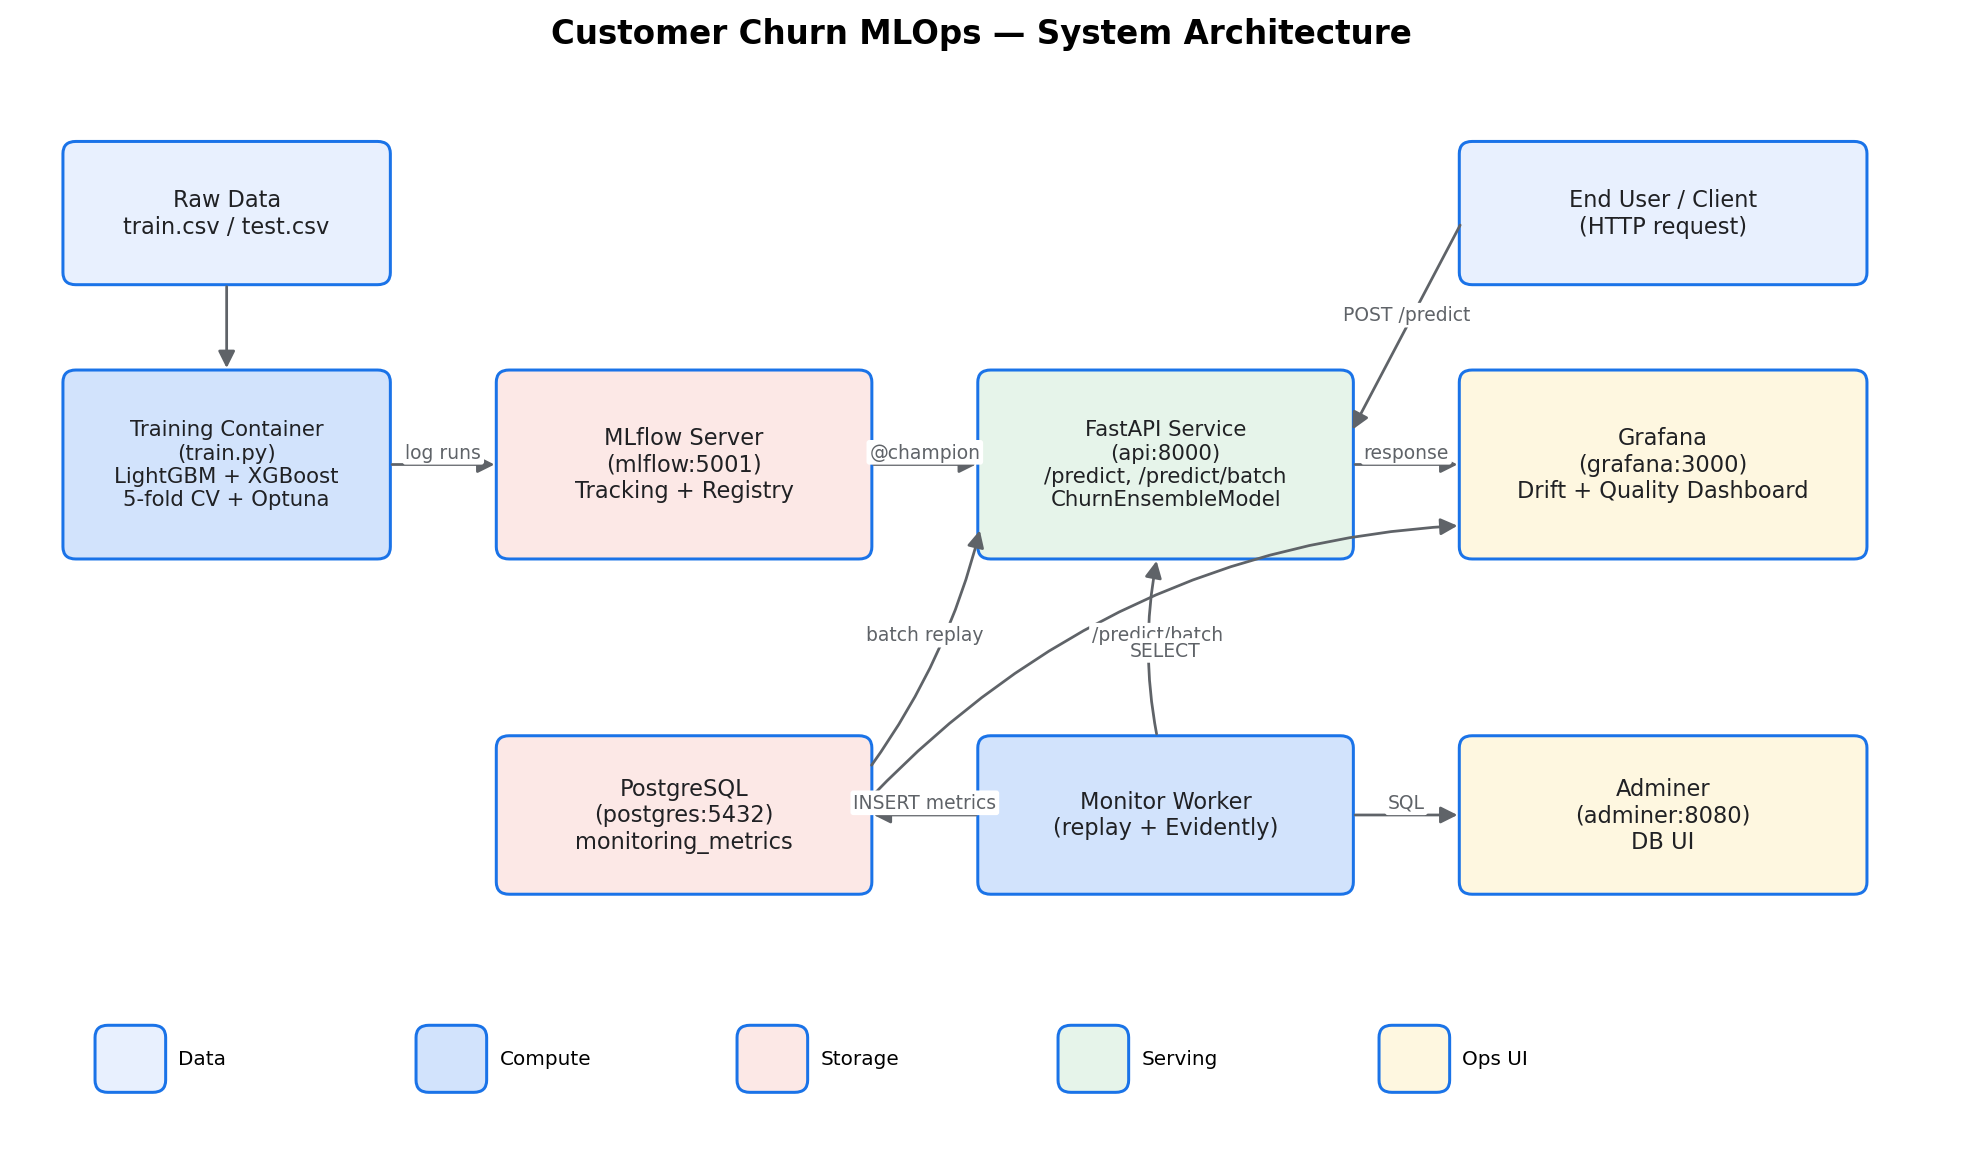
\includegraphics[width=0.95\textwidth]{fig_architecture.png}
  \caption{System architecture. Boxes are Docker Compose services;
           arrows show data and control flow. Service-name DNS resolves
           inside the Compose network (e.g.,
           \texttt{mlflow:5001}); host ports are published for the UIs
           (e.g.,
           \texttt{localhost:5001} for MLflow,
           \texttt{localhost:3000} for Grafana).}
  \label{fig:arch}
\end{figure*}

Figure~\ref{fig:arch} shows the six Docker Compose services that make
up the runtime: the FastAPI prediction \texttt{api}, the
\texttt{mlflow} tracking server, a \texttt{postgres} metrics database,
the \texttt{grafana} visualisation server, an \texttt{adminer} database
UI for ad-hoc inspection, and the \texttt{monitor} replay worker.
Training is performed in a separate container (or directly on the host
during development) that reads the dataset and writes runs into the
MLflow tracking store. The serving and training stages share a single
artefact contract---a registered model named
\texttt{CustomerChurnEnsemble} carrying an alias
\texttt{@champion}---which decouples the model's identity from its
underlying version number and is the single point of integration
between training and serving.

\paragraph{Network boundary} An onboarding pitfall worth emphasising
early is that two URL spaces coexist: inside the Compose network
services address each other by service name (e.g., the API uses
\texttt{MLFLOW\_TRACKING\_URI=http://mlflow:5001}), while a developer
on the host machine reaches the same services via published
\texttt{localhost} ports (5001, 8000, 3000, 8080). Misconfiguring this
boundary is the most common cause of first-run errors.

\paragraph{Tool inventory} Table~\ref{tab:tools} lists every
third-party tool in the stack together with the role it plays in this
project. Versions are pinned in \texttt{pyproject.toml} and the
\texttt{docker-compose.yml} file.

\begin{table*}[t]
\caption{Tool inventory and per-tool role in the pipeline.}
\label{tab:tools}
\centering\small
\begin{tabularx}{\textwidth}{@{}llX@{}}
\toprule
\textbf{Tool} & \textbf{Version} & \textbf{Role in this project} \\
\midrule
LightGBM       & 4.6.0   & First gradient-boosting learner; 5 fold models per pipeline run. \\
XGBoost        & 3.2.0   & Second gradient-boosting learner averaged with LightGBM at inference. \\
scikit-learn   & 1.x     & Stratified $K$-fold splitter, classification metrics, baseline utilities. \\
Optuna         & 4.7.0   & Bayesian (TPE) hyper-parameter optimisation; studies persisted in SQLite. \\
MLflow         & 3.10.0  & Experiment tracking, artefact store, model registry and alias-based promotion. \\
FastAPI        & 0.135.1 & ASGI web framework hosting the prediction endpoints. \\
Pydantic       & 2.x     & Request/response schema validation at the API boundary. \\
Uvicorn        & --      & ASGI server in the API container. \\
joblib         & --      & Serialisation of the per-fold sklearn-compatible boosters inside the pyfunc wrapper. \\
Evidently      & 0.7.21  & Drift and classification quality reports computed batch-by-batch by the monitor. \\
PostgreSQL     & 16      & Storage backend for the \texttt{monitoring\_metrics} table read by Grafana. \\
psycopg / psycopg2 & 3.3.3 / 2.9.12 & Python clients used by the monitor and Grafana datasource respectively. \\
Grafana        & 11.3.0  & Eight-panel monitoring dashboard, provisioned from JSON. \\
Adminer        & 5       & Web UI for ad-hoc inspection of the metrics database. \\
pandas / NumPy & --      & Data loading and tensor manipulation throughout. \\
matplotlib / seaborn & -- & Feature importance plots, confusion matrices and EDA figures. \\
Docker, Docker Compose & --     & Container build and multi-service orchestration. \\
uv             & --      & Fast dependency resolver used by all CI workflows. \\
Ruff           & 0.15.5  & Linting (gating) and formatting (advisory) in CI. \\
Pytest, pytest-cov & 8.3.0 / 5.0.0 & Test runner and coverage measurement with a 50\% floor. \\
httpx          & 0.28.0  & In-process HTTP client used by the FastAPI test client. \\
pip-audit      & 2.7.3   & Supply-chain vulnerability scanning of the resolved environment. \\
Gitleaks       & --      & Pre-merge and weekly secret scanning, reporting to GitHub's code-scanning UI. \\
GitHub Actions & --      & Five workflows: \texttt{ci}, \texttt{docker}, \texttt{release}, \texttt{secret-scan}, \texttt{train}. \\
CodeQL         & --      & Static-analysis security scanning via GitHub's default setup. \\
\bottomrule
\end{tabularx}
\end{table*}

% ===========================================================================
\section{Data and Feature Engineering}\label{sec:data}

The pipeline consumes the IBM Telco customer-churn dataset, expanded by
augmentation to roughly 600\,k rows for training and a separately
provided unlabelled test set. The schema contains a mixture of
numerical attributes (\texttt{tenure}, \texttt{MonthlyCharges},
\texttt{TotalCharges}, \texttt{SeniorCitizen}) and categorical
attributes describing services subscribed (phone, internet, streaming,
add-on protection) plus contractual and payment information. The
target is the binary indicator \texttt{Churn}.

\begin{figure}[t]
  \centering
  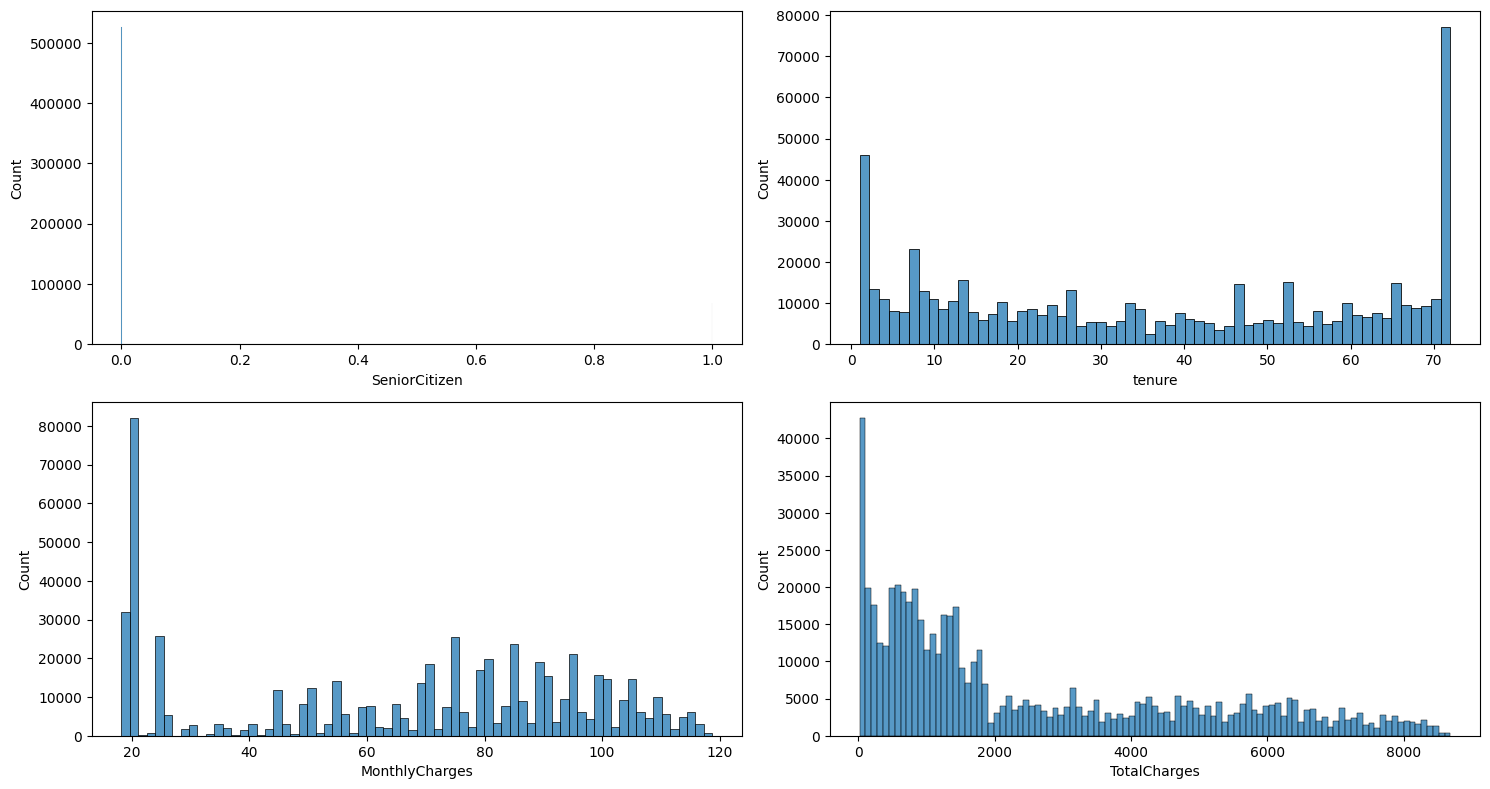
\includegraphics[width=\linewidth]{numeric_distributions.png}
  \caption{Marginal distributions of the four numeric attributes.
           \texttt{tenure} is bimodal (recently-joined customers and
           long-tenured stayers), \texttt{MonthlyCharges} clusters
           around the price points of the bundled tariffs, and
           \texttt{TotalCharges} is heavily right-skewed.}
  \label{fig:numeric}
\end{figure}

\begin{figure}[t]
  \centering
  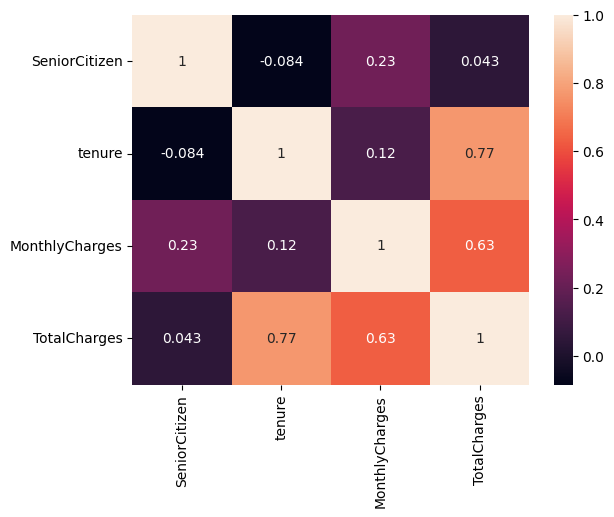
\includegraphics[width=\linewidth]{correlation_heatmap.png}
  \caption{Pearson correlation between numeric features. The strong
           correlation between \texttt{tenure} and \texttt{TotalCharges}
           (0.77) motivates the derived feature \texttt{AvgMonthlyCharge}
           introduced in Section~\ref{sec:data}.}
  \label{fig:corr}
\end{figure}

\begin{figure}[t]
  \centering
  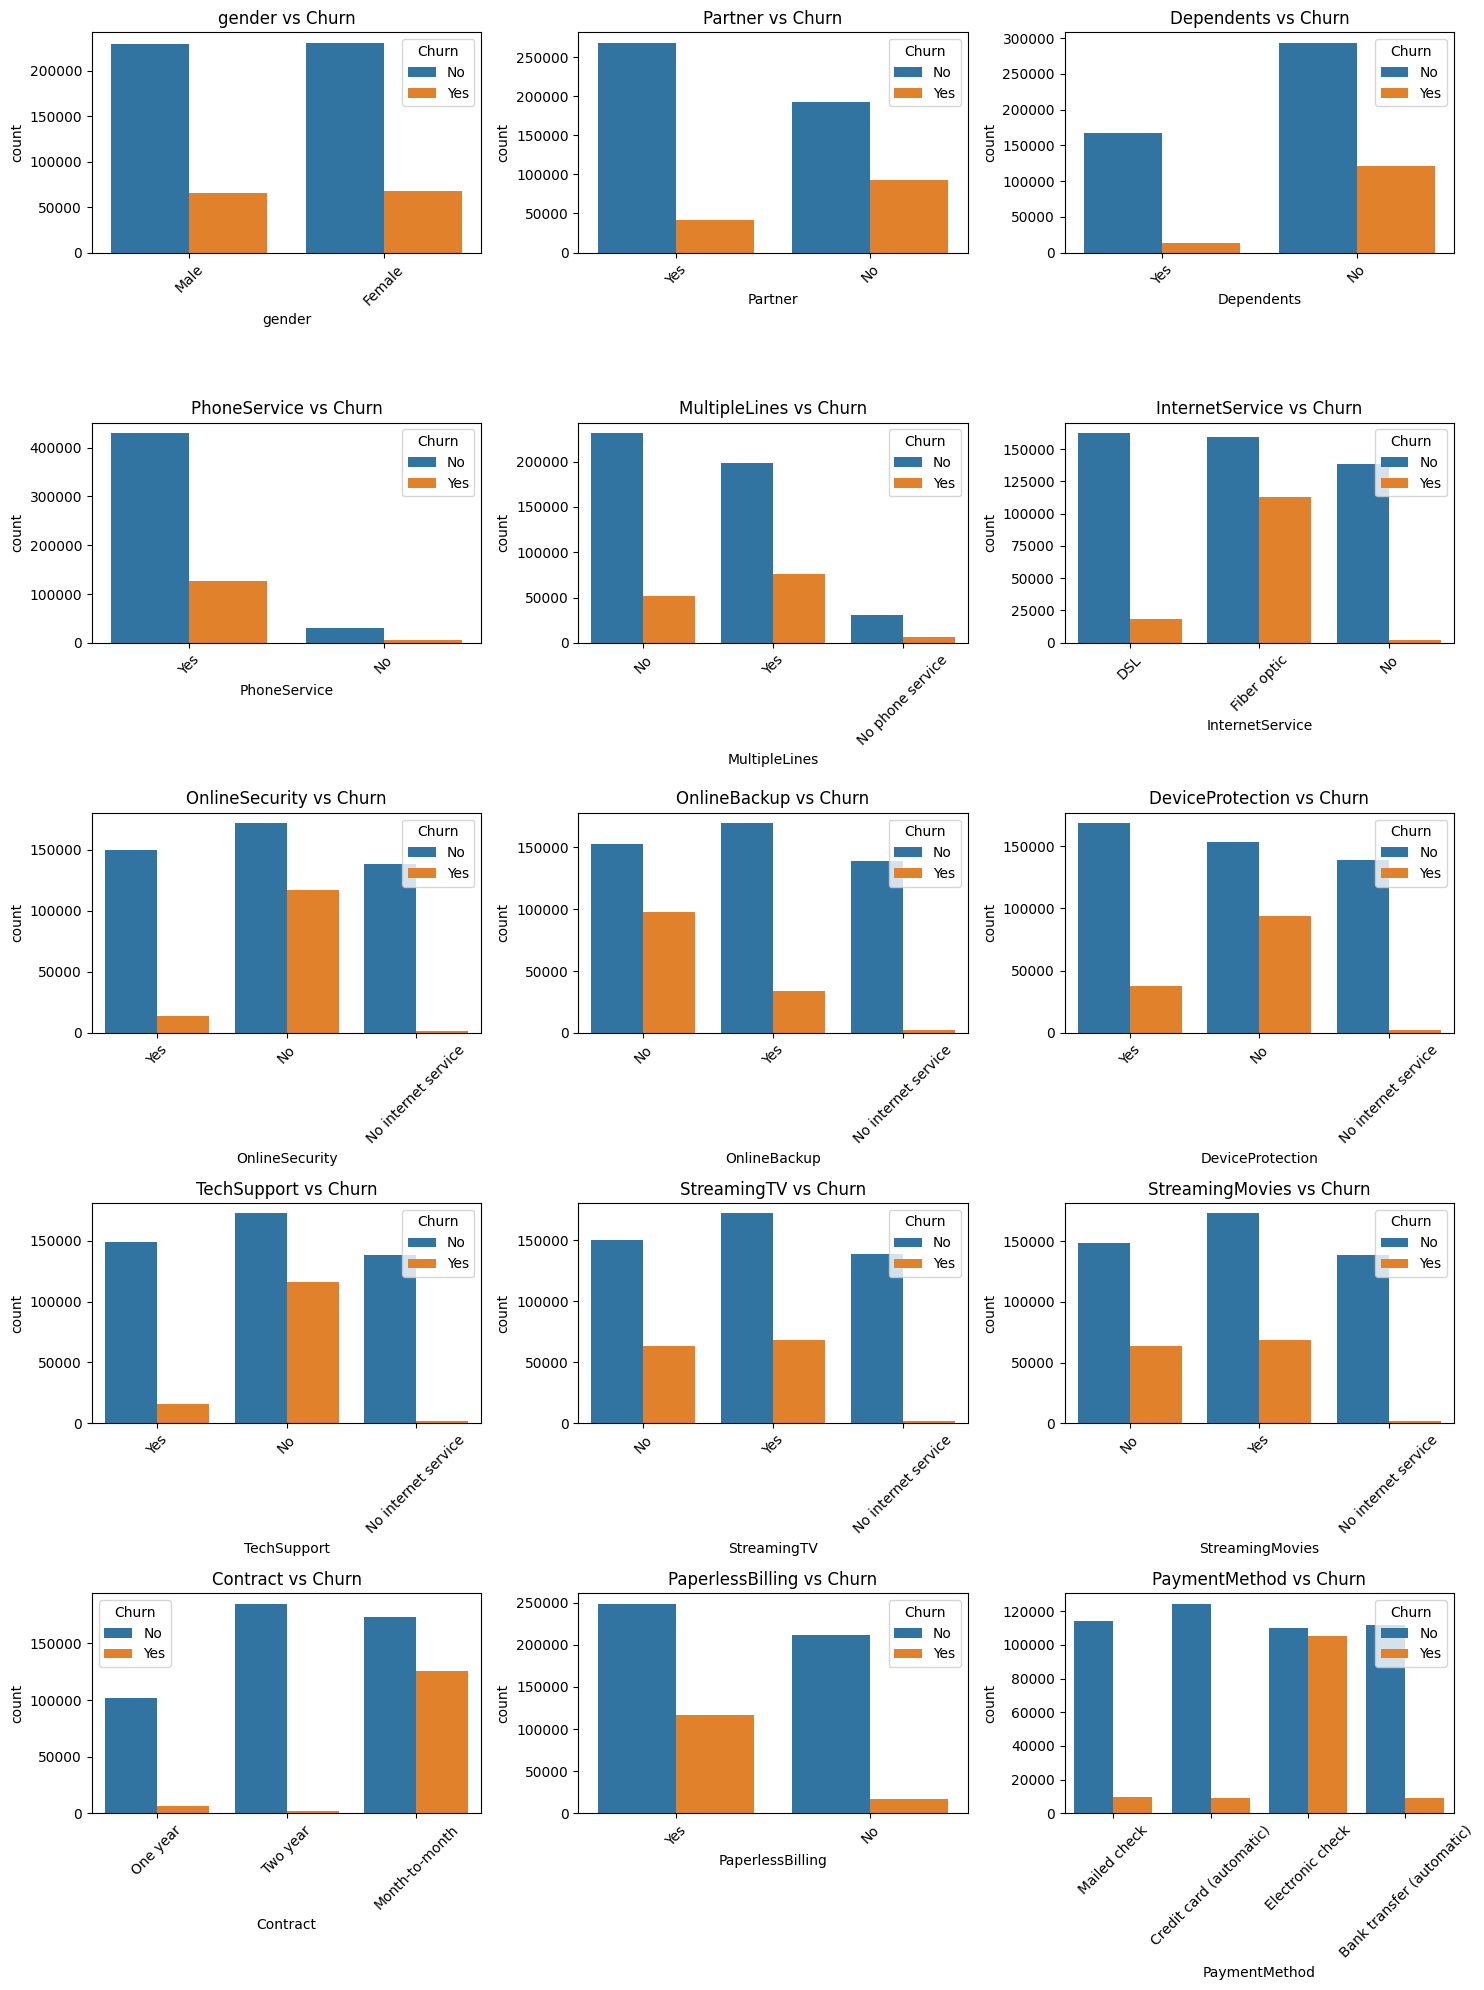
\includegraphics[width=\linewidth]{categorical_vs_churn.png}
  \caption{Churn rate by categorical attribute. Month-to-month
           contracts, fibre-optic internet and electronic-check payments
           show markedly elevated churn relative to other levels.}
  \label{fig:cat}
\end{figure}

\paragraph{Derived features} Two derived features are added to the raw
schema. \texttt{AvgMonthlyCharge} is computed as
\texttt{TotalCharges/tenure} (with zero-tenure guard); it disentangles
total revenue from tenure length and is therefore a less collinear
signal than its components (Figure~\ref{fig:corr}).
\texttt{TotalServices} is the count of subscribed add-on services per
customer; it summarises the breadth of the customer's relationship with
the operator in a single integer.

\paragraph{Encoding} Categorical attributes with more than two levels
are one-hot encoded; binary categorical attributes (e.g.,
\texttt{Partner}, \texttt{PaperlessBilling}) are mapped to \{0,1\}; the
\texttt{gender} column is dropped as it carries no discriminative signal
on this dataset and is excluded for fairness considerations. The final
feature list is persisted alongside the model in the MLflow registry to
guarantee column-order parity at serving time.

\paragraph{Split} A stratified split preserves the empirical churn rate
in every cross-validation fold; the monitor service later re-uses the
same stratified split, holding out 20\,\% of the training set as a
``reference'' distribution against which incoming batches are compared.

% ===========================================================================
\section{Training Pipeline}\label{sec:training}

\begin{figure*}[t]
  \centering
  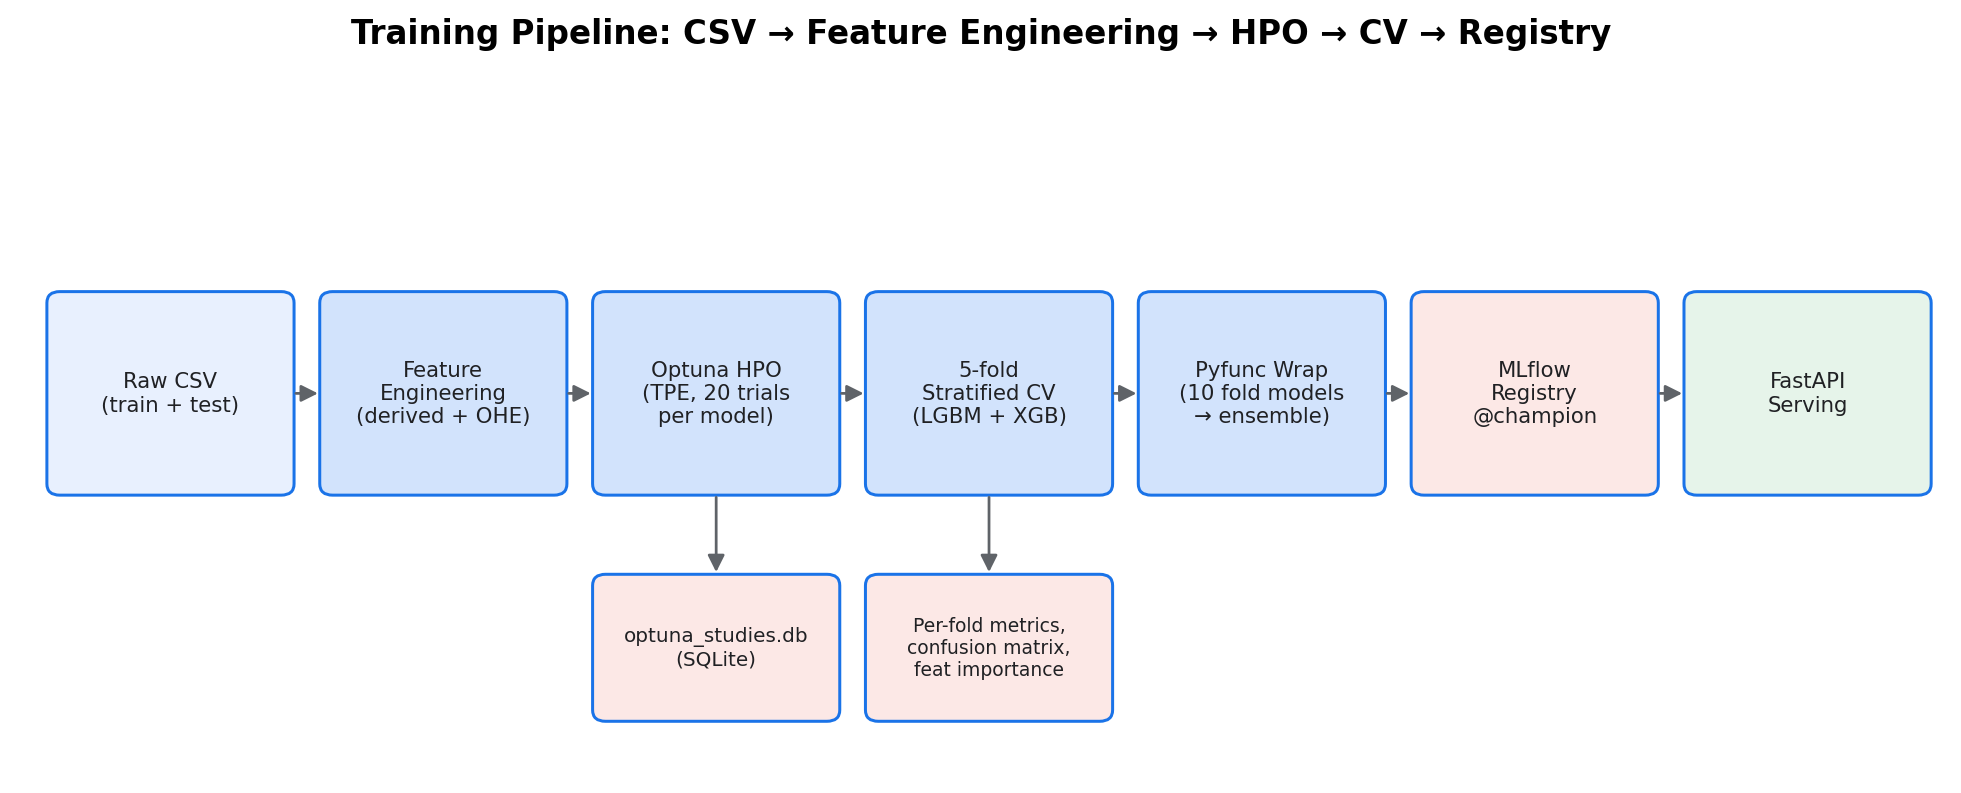
\includegraphics[width=0.95\textwidth]{fig_training_pipeline.png}
  \caption{Training pipeline. Raw CSV is feature-engineered, the
           hyper-parameters of each base learner are tuned by Optuna,
           five-fold stratified cross-validation produces ten fold
           models (five LightGBM + five XGBoost) that are packaged into
           a single \texttt{pyfunc} ensemble and registered in MLflow
           under the alias \texttt{@champion}.}
  \label{fig:trainpipe}
\end{figure*}

The training stage is implemented in \texttt{train.py} and is
visualised in Figure~\ref{fig:trainpipe}. It proceeds in five logical
phases.

\paragraph{Phase 1 -- Hyper-parameter optimisation} Two independent
Optuna studies (one per base learner) are run for a configurable
number of trials, persisting to \texttt{optuna\_studies.db} so that
interrupted runs can resume and so that the search history can be
inspected post-hoc. For each trial Optuna samples a candidate
configuration from the search space (e.g., \texttt{learning\_rate},
\texttt{num\_leaves}, \texttt{max\_depth}, regularisation strengths)
and scores it with a single hold-out evaluation of the validation
AUC.

\paragraph{Phase 2 -- Stratified cross-validation} The best
hyper-parameter set per base learner is then refit five times under
stratified five-fold cross-validation. Each fold trains both a
LightGBM and an XGBoost model on the same training partition,
yielding ten fold-level models in total. Validation AUC, F1, accuracy,
precision, recall and log-loss are recorded per fold.

\begin{figure}[t]
  \centering
  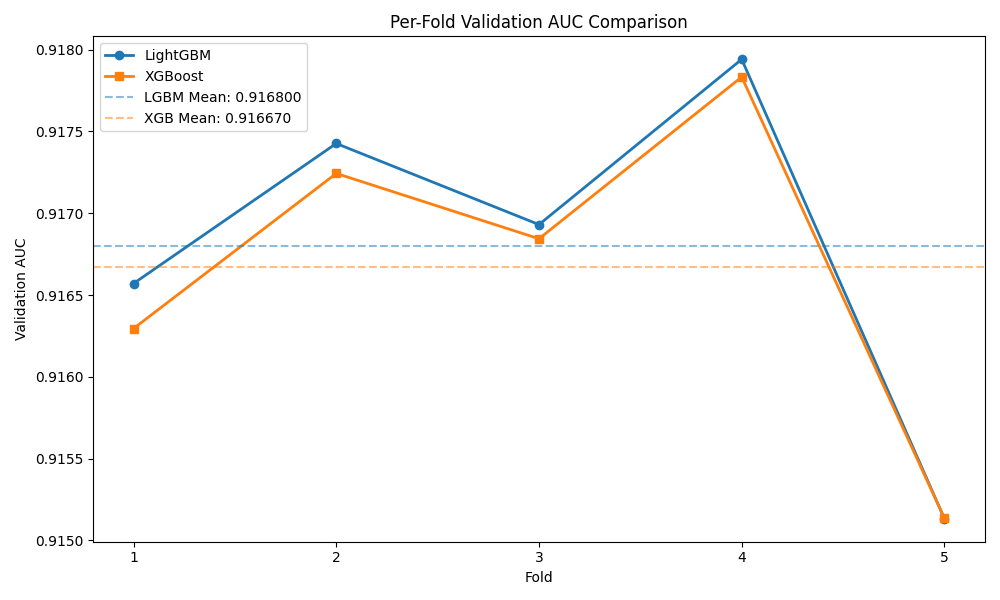
\includegraphics[width=\linewidth]{cv_auc_comparison.png}
  \caption{Per-fold validation AUC of LightGBM and XGBoost. The two
           learners track each other closely (mean AUC differs in the
           fourth decimal), supporting the use of a simple
           equal-weight average rather than a learned stacker.}
  \label{fig:cvauc}
\end{figure}

\paragraph{Phase 3 -- Ensemble assembly} The ten fold models are
wrapped inside a custom \texttt{pyfunc} class
(\texttt{ChurnEnsembleModel}) whose
\texttt{predict()} method (i) reindexes the incoming feature frame to
the persisted column order, (ii) averages the five LightGBM
probabilities, (iii) averages the five XGBoost probabilities, and (iv)
returns the mean of the two means. Wrapping all fold models inside a
single registry entity keeps the registry surface area small and
guarantees atomic promotion.

\begin{figure}[t]
  \centering
  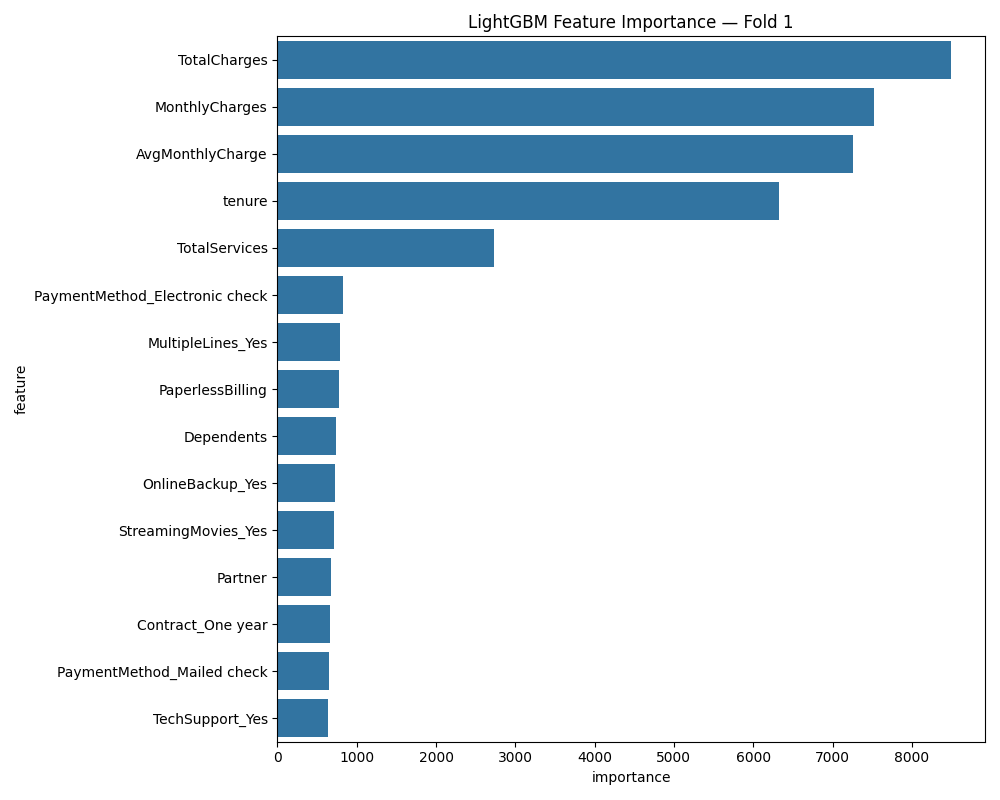
\includegraphics[width=\linewidth]{lgbm_feature_importance.png}
  \caption{LightGBM gain-based feature importance for fold~1. The four
           strongest signals are the numeric charge/tenure attributes
           and the derived \texttt{AvgMonthlyCharge}, which dominate
           the long tail of one-hot indicators.}
  \label{fig:lgbmimp}
\end{figure}

\begin{figure}[t]
  \centering
  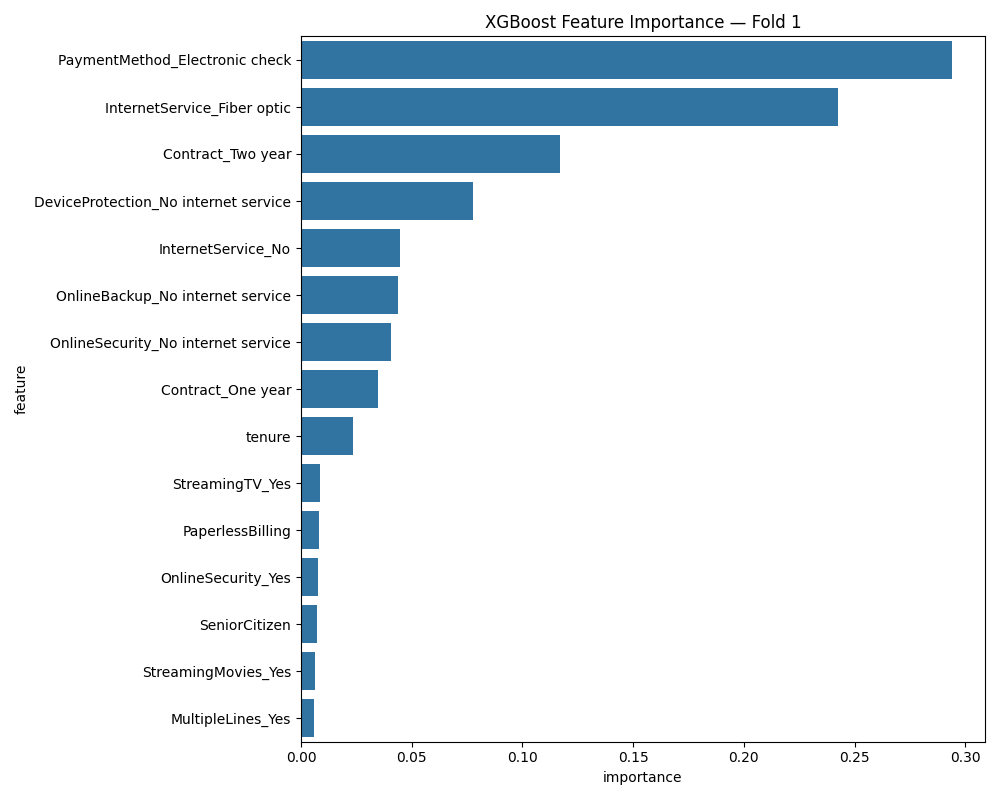
\includegraphics[width=\linewidth]{xgb_feature_importance.png}
  \caption{XGBoost gain-based feature importance for fold~1. The
           ranking corroborates the LightGBM picture: the same four
           features dominate but with a different magnitude profile,
           illustrating why averaging the two learners is preferable to
           using either one alone.}
  \label{fig:xgbimp}
\end{figure}

\paragraph{Phase 4 -- MLflow logging} Each training run produces a
parent MLflow run with ten nested child runs (one per fold-learner
combination). The parent run records aggregate metrics and the
serialised ensemble; child runs carry per-fold metrics, the per-fold
confusion matrix as a PNG artefact (Figures~\ref{fig:lgbmcm}
and~\ref{fig:xgbcm}), and the per-fold feature-importance plot.

\begin{figure}[t]
  \centering
  \begin{subfigure}[t]{\linewidth}
    \centering
    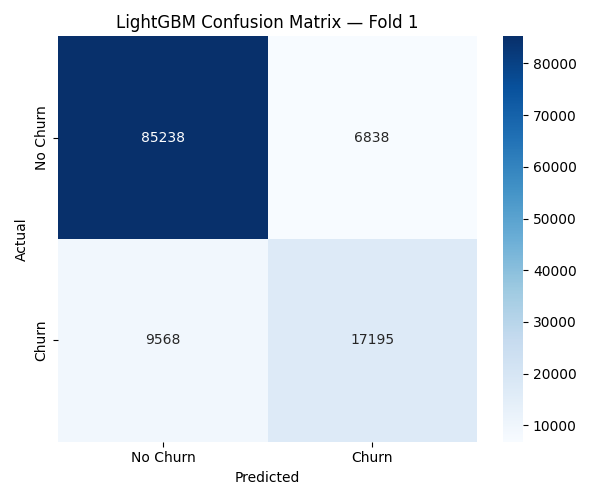
\includegraphics[width=0.78\linewidth]{lgbm_confusion_matrix.png}
    \caption{LightGBM, fold 1.}
    \label{fig:lgbmcm}
  \end{subfigure}\vspace{0.3em}
  \begin{subfigure}[t]{\linewidth}
    \centering
    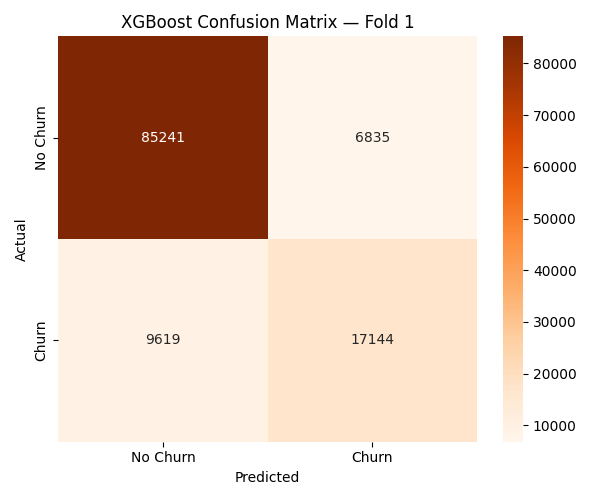
\includegraphics[width=0.78\linewidth]{xgb_confusion_matrix.png}
    \caption{XGBoost, fold 1.}
    \label{fig:xgbcm}
  \end{subfigure}
  \caption{Per-fold confusion matrices logged to MLflow. Classes are
           imbalanced (roughly 1:3) so the operating threshold is
           tuned downstream from these matrices.}
\end{figure}

\paragraph{Phase 5 -- Registry promotion} After successful completion
the parent run is registered under the name
\texttt{CustomerChurnEnsemble}; the operator (or, in future work, an
automated gate) attaches the \texttt{@champion} alias to the new
version, which is the version subsequently loaded by the serving
container at start-up.

\begin{figure}[t]
  \centering
  \screenshot{screenshot_mlflow_registry.png}{\linewidth}{MLflow
    Registry view of \texttt{CustomerChurnEnsemble} with the
    \texttt{@champion} alias visible.}
  \caption{MLflow registry view. Capture from
           \url{http://localhost:5001} once a training run has been
           promoted.}
  \label{fig:mlflowreg}
\end{figure}

\begin{figure}[t]
  \centering
  \screenshot{screenshot_mlflow_run.png}{\linewidth}{One MLflow
    run page showing parent + 10 nested child runs (metrics tab open).}
  \caption{MLflow run detail. Parent run with nested child runs and
           per-fold metrics; see Phases 2--4 above.}
  \label{fig:mlflowrun}
\end{figure}

\paragraph{Score distribution} Figure~\ref{fig:scoredist} shows the
distribution of ensemble churn probabilities on the held-out test set.
The mass is concentrated near zero (the majority class) with a
long tail towards one, justifying the use of AUC and log-loss as
primary metrics rather than raw accuracy.

\begin{figure}[t]
  \centering
  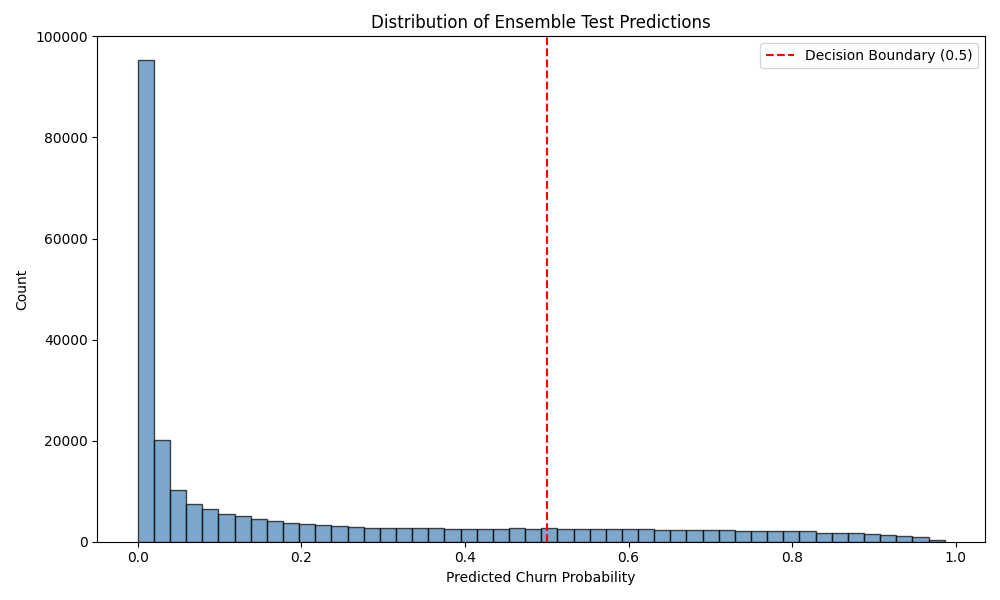
\includegraphics[width=\linewidth]{ensemble_prediction_distribution.png}
  \caption{Distribution of ensemble churn probabilities on the
           held-out test set. The red dashed line marks the default
           0.5 decision boundary.}
  \label{fig:scoredist}
\end{figure}

% ===========================================================================
\section{Serving Layer (FastAPI)}\label{sec:serving}

The serving layer is a FastAPI application (\texttt{web\_service.py})
that loads the model at start-up and exposes four endpoints:
\texttt{GET\,/} (health), \texttt{POST\,/predict} for a single
customer, \texttt{POST\,/predict/batch} for an array of customers, and
\texttt{GET\,/model/info} which returns the loaded MLflow version
metadata. Requests and responses are typed by Pydantic models defined
in \texttt{schemas/schemas.py}; six enumerations enforce the legal
values of categorical fields (e.g., \texttt{Contract},
\texttt{PaymentMethod}, \texttt{InternetService}) and bounded numeric
constraints catch out-of-range \texttt{tenure} or charges before they
reach the model.

\paragraph{Train/serve parity} A frequent failure mode of deployed
classifiers is feature-engineering drift between training and serving.
This system addresses the risk by re-implementing the training-time
transformations inside the API in a function whose only inputs are the
validated Pydantic payload and the persisted feature list. The
function performs (i) enum-to-binary mapping for \texttt{YesNo}
fields, (ii) one-hot encoding of multi-level categoricals, (iii)
re-derivation of \texttt{AvgMonthlyCharge} and \texttt{TotalServices},
and (iv) reindexing onto the canonical column order persisted with the
model. Defects introduced by hand-maintaining this parity are
discussed in Section~\ref{sec:lessons}.

\paragraph{Container path resolution} A small helper translates the
host-relative MLflow artefact paths recorded inside
\texttt{mlruns/} into the in-container paths used at run time. Without
this translation the API would attempt to read artefacts at the
filesystem location they happened to occupy on the developer's laptop.

\begin{figure}[t]
  \centering
  \screenshot{screenshot_fastapi_swagger.png}{\linewidth}{Swagger UI
    listing GET /, POST /predict, POST /predict/batch, GET /model/info.}
  \caption{Auto-generated Swagger UI for the prediction service at
           \url{http://localhost:8000/docs}.}
  \label{fig:swagger}
\end{figure}

\begin{figure}[t]
  \centering
  \screenshot{screenshot_fastapi_response.png}{\linewidth}{Example
    POST /predict request and response, showing churn\_probability
    and prediction fields.}
  \caption{Example single-customer prediction round-trip via the
           Swagger ``Try it out'' panel.}
  \label{fig:swaggerexample}
\end{figure}

% ===========================================================================
\section{Monitoring and Drift Detection}\label{sec:monitoring}

The monitoring component is a long-running container
(\texttt{monitor.py}) that replays both the labelled hold-out
(``reference'') and the unlabelled test stream through the serving API
in fixed-size batches at a fixed cadence (defaults: batch size~1\,000,
interval~10\,s, configurable through environment variables). For each
batch the worker (i) collects the churn probabilities returned by the
API, (ii) constructs an Evidently \texttt{Report} that includes a
dataset-level drift metric, a per-column drift metric on the
prediction distribution, and (when labels are available) classification
quality metrics, and (iii) inserts a single row into the
\texttt{monitoring\_metrics} table in Postgres. Eight
Grafana~\cite{grafana_docs} panels read from that table and refresh on
a five-second interval.

\paragraph{Drift definition} The dataset-level metric reports the
number of input columns whose distribution has drifted relative to the
reference fold, using Evidently's default per-type detectors (Jensen--
Shannon distance for numeric features, Wasserstein for ordinal,
chi-squared for categorical). The prediction-drift metric uses
Population Stability Index on the predicted-probability histogram.
A column is considered drifted when its detector's p-value falls below
the standard 0.05 threshold; the share of drifted columns is the
primary drift health indicator displayed in red on the dashboard.

\paragraph{Synthetic drift injection} For demonstration and stress
testing, the worker can inject synthetic drift into the test stream
through three modes (\texttt{gradual}, \texttt{sustained},
\texttt{cycle}) controlled by environment variables. The injector
amplifies a configurable subset of numerical features by an intensity
that varies over batches; the resulting drift signal then propagates
through the monitor, Postgres and Grafana so that the visualisations
become observably reactive.

\begin{figure}[t]
  \centering
  \screenshot{screenshot_grafana_dashboard.png}{\linewidth}{Customer
    Churn Monitoring dashboard with all eight panels populated.}
  \caption{Grafana monitoring dashboard. Anonymous viewer access is
           enabled in the provisioning so reviewers can open
           \url{http://localhost:3000} without authentication.}
  \label{fig:grafana}
\end{figure}

\begin{figure}[t]
  \centering
  \screenshot{screenshot_grafana_drift.png}{\linewidth}{Close-up of
    the Drifted Columns and Share of Drifted Columns time-series
    panels with synthetic drift enabled.}
  \caption{Effect of the \texttt{DRIFT\_MODE=gradual} synthetic drift
           injection on the dashboard's drift panels.}
  \label{fig:gradualdrift}
\end{figure}

\begin{figure}[t]
  \centering
  \screenshot{screenshot_adminer.png}{\linewidth}{Adminer table view
    of \texttt{monitoring\_metrics} showing recent rows.}
  \caption{Adminer view of the metrics table that backs the dashboard.
           Useful for verifying that the monitor is actually writing
           rows when the dashboard appears empty.}
  \label{fig:adminer}
\end{figure}

% ===========================================================================
\section{Testing, CI/CD and Supply-Chain Security}\label{sec:cicd}

\subsection{Test suite}
The pytest suite in \texttt{project/tests/} is organised in three
layers. \texttt{test\_schemas.py} exercises the Pydantic validation
rules to catch schema regressions (eight tests over enum membership,
field constraints and response serialisation).
\texttt{test\_web\_service.py} drives the FastAPI app through
\texttt{TestClient}, substituting the registry-backed model with a
\texttt{\_StubChurnModel} fixture that always returns probability~0.42;
this isolates the endpoint, preprocessing and response-shaping logic
from MLflow availability. \texttt{test\_monitor.py} verifies the
synthetic drift injector's intensity scheduling and the CSV-to-API
feature transformation. A 50\,\% coverage floor is enforced in CI;
\texttt{train.py} and the Grafana provisioning are intentionally
omitted from the measured surface because they are exercised by the
\texttt{train.yml} workflow rather than by pytest.

\subsection{CI/CD pipeline}
Figure~\ref{fig:cicd} summarises the five GitHub Actions workflows.

\begin{figure*}[t]
  \centering
  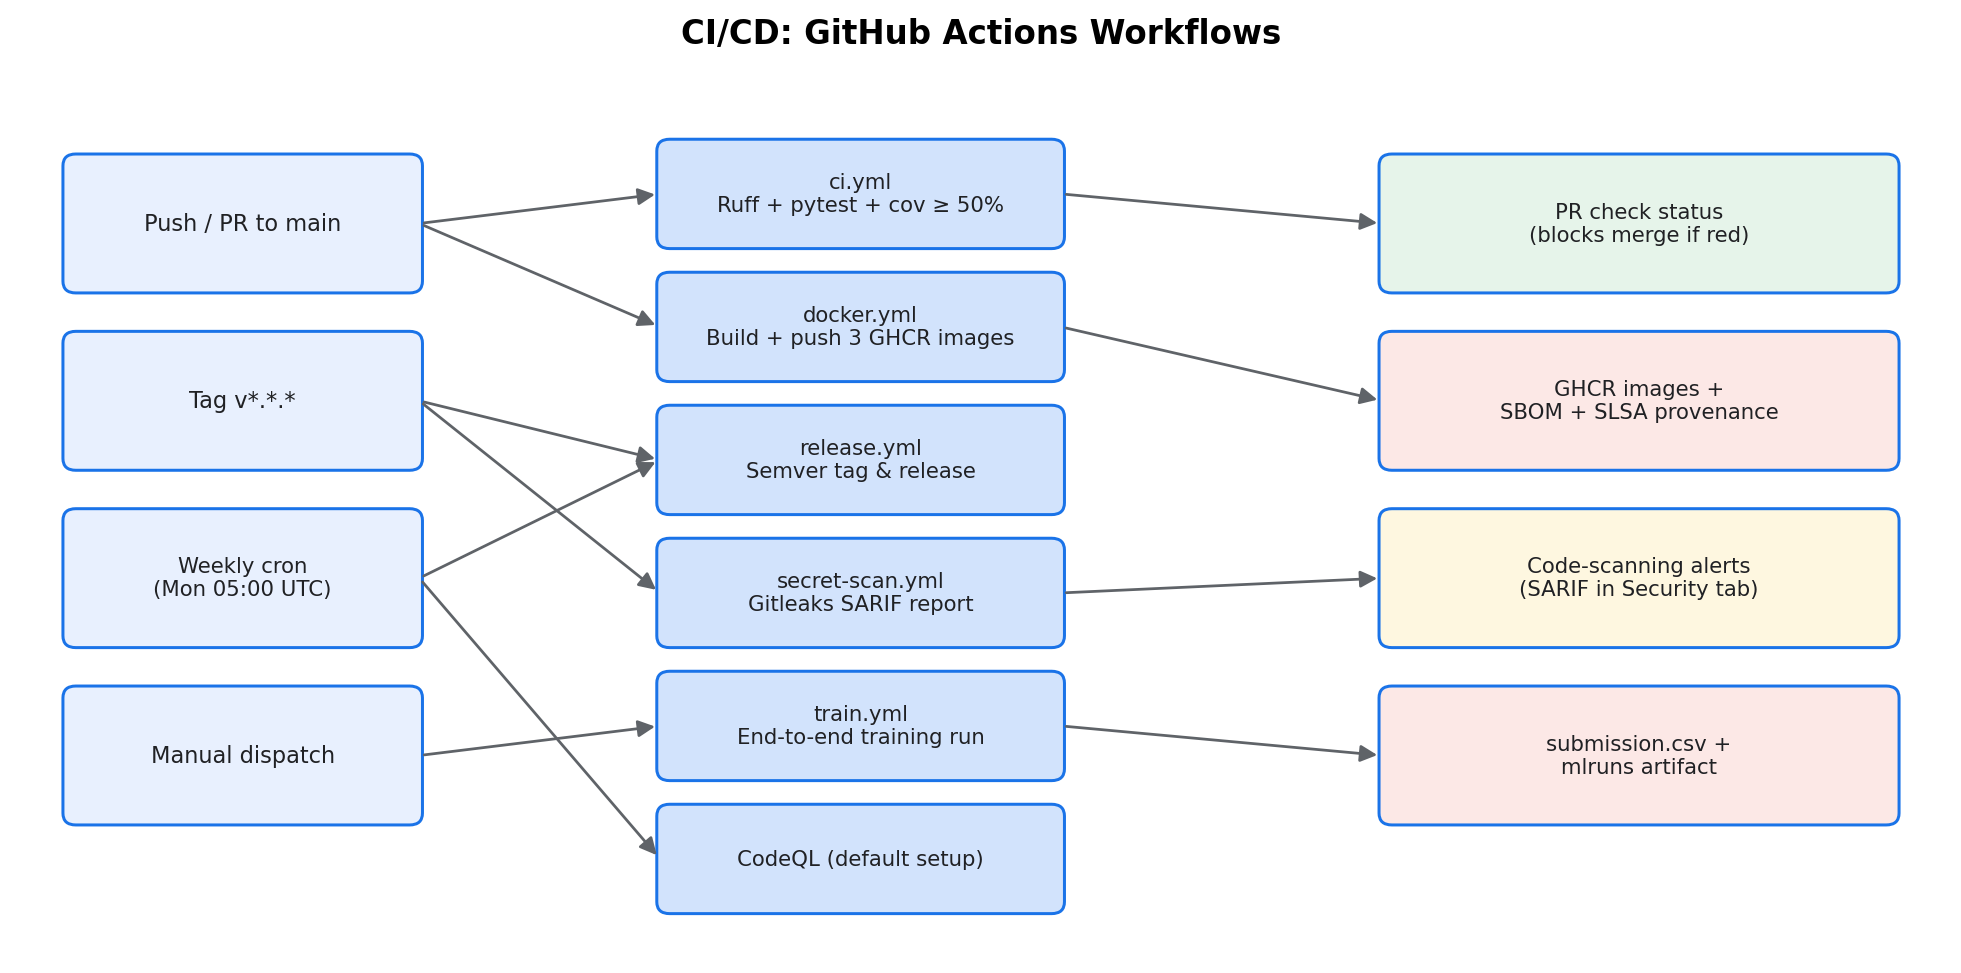
\includegraphics[width=0.95\textwidth]{fig_cicd.png}
  \caption{GitHub Actions topology. Triggers on the left, workflows in
           the middle, observable outputs on the right.}
  \label{fig:cicd}
\end{figure*}

\begin{itemize}
  \item \textbf{ci.yml}---runs on every push and PR to \texttt{main};
        executes Ruff (lint as hard gate, format check advisory),
        Pytest with a coverage gate and uploads a coverage XML artefact.
  \item \textbf{docker.yml}---runs on push to \texttt{main}, semver
        tags and PRs; builds the three production images (\texttt{api},
        \texttt{mlflow}, \texttt{monitor}) and pushes them to GHCR with
        a CycloneDX SBOM and SLSA~v1 provenance
        attestation~\cite{slsa_v1}.
  \item \textbf{release.yml}---re-tags GHCR images and publishes a
        GitHub release on each semver tag.
  \item \textbf{secret-scan.yml}---runs Gitleaks on every push,
        every PR to \texttt{main} and on a weekly cron (Monday 05:00
        UTC); findings appear as SARIF reports in GitHub's
        code-scanning UI and block PRs.
  \item \textbf{train.yml}---manual dispatch; performs an end-to-end
        training run with a temporary MLflow server, uploads
        \texttt{submission.csv} and the entire \texttt{mlruns}
        directory as workflow artefacts so that registered models can
        be inspected without rebuilding the environment locally.
\end{itemize}

CodeQL static analysis is enabled through GitHub's \emph{default
setup} (Settings $\to$ Code security $\to$ Code scanning) rather than
via a workflow file; the results surface alongside Gitleaks alerts in
the repository's Security tab. The combination of CodeQL,
\texttt{pip-audit} (dependency vulnerabilities) and Gitleaks (secret
hygiene) provides three independent channels of supply-chain
assurance.

\begin{figure}[t]
  \centering
  \screenshot{screenshot_github_actions.png}{\linewidth}{Actions tab
    of the repository showing a successful PR run with green status on
    ci.yml, docker.yml and secret-scan.yml.}
  \caption{GitHub Actions run summary for a representative PR.}
  \label{fig:gha}
\end{figure}

% ===========================================================================
\section{Lessons Learnt}\label{sec:lessons}

The following observations crystallised during construction of the
pipeline; they are reported here because they were the design-time
decisions that proved most consequential.

\paragraph{1. Hand-mirrored preprocessing is the dominant train/serve
risk}
The serving layer re-implements the training-time feature engineering
rather than serialising a scikit-learn \texttt{Pipeline} object. This
keeps the deployed image small and avoids version-pinning the entire
sklearn tree, but it makes the equality of the two implementations a
manual invariant. The mitigations adopted---persisting the feature list
inside the registered model, validating the API with the same payloads
the training code emits, and unit-testing the preprocessor---are
defensible but not sufficient. A safer long-term design is to serialise
a single sklearn or
\texttt{FunctionTransformer} pipeline inside the
\texttt{pyfunc} wrapper.

\paragraph{2. Wrapping all fold models in a single registry entity is
worth the memory cost}
Promoting ten fold models behind a single \texttt{@champion} alias
makes deployment atomic and rolls forward and back as one unit. The
cost is that the deployed container holds ten boosters in memory; for
this scale (small, tabular) the trade-off is favourable, but it would
not extrapolate to deep-learning ensembles without a more sophisticated
serving topology.

\paragraph{3. The 50\,\% coverage floor reflects a deliberate scope
choice, not laziness}
Coverage measurement intentionally excludes \texttt{train.py} because
training is exercised end-to-end by the \texttt{train.yml} workflow
rather than by pytest. Lowering the floor to 50\,\% prevents the gate
from rewarding shallow tests written purely to pad the percentage and
keeps the rule honest.

\paragraph{4. The service-name versus \texttt{localhost} boundary is
the most common onboarding stumble}
Two URL spaces---intra-network DNS (\texttt{mlflow:5001}) and host
ports (\texttt{localhost:5001})---coexist throughout the codebase. Any
new contributor will encounter this distinction at least once, and it
is the source of nearly every ``works on my machine'' incident on the
project. The repository's \texttt{CLAUDE.md} now documents the
distinction explicitly.

\paragraph{5. A self-hosted Evidently + Postgres + Grafana monitor is
viable at this scale}
Production teams often default to a managed observability product,
but the requirements of an MLOps reference implementation---
auditability, offline operation, full control over the schema---are
better served by the lightweight self-hosted alternative used here.
The eight-panel dashboard, the synthetic drift injector and the
Postgres schema together account for less than 1\,000 lines of code.

\paragraph{6. SLSA v1 attestations are cheap once the build is in
Actions}
Adding SBOM generation and SLSA provenance to the container build was
a one-line addition once the workflow was already publishing to GHCR.
The marginal cost is small and the resulting supply-chain story is
much easier to defend than ``trust the image''.

% ===========================================================================
\section{Future Works}\label{sec:future}

Five directions naturally extend this work:
\begin{enumerate}
  \item \textbf{Workflow orchestration with Prefect.} The presence of
        an empty \texttt{project/prefect-data/} directory in the
        repository suggests this was already scoped; replacing the
        ad-hoc batch loop in the monitor with Prefect flows would
        give first-class scheduling, retries and observability.
  \item \textbf{Automated champion--challenger gate.} The
        \texttt{@champion} alias is presently moved manually; a gate
        inside \texttt{train.py} that compares the new candidate to
        the incumbent on a frozen validation slice (with a confidence
        interval) would close the loop and remove a manual step.
  \item \textbf{Per-customer explainability via SHAP.}
        Lundberg and Lee~\cite{lundberg2017shap} give a unified
        framework for attributing a prediction to its features; adding
        SHAP values to the \texttt{/predict} response would turn the
        service from a black-box classifier into a decision-support
        tool for retention agents.
  \item \textbf{Alert-driven rollback.} A Grafana alert wired into a
        small operator could move the \texttt{@champion} alias back
        to the previous version when the drift or quality panels cross
        a threshold; this would make the loop fully self-healing.
  \item \textbf{Canary serving.} Running two FastAPI replicas behind a
        weighted reverse proxy would allow new champion candidates to
        be A/B-tested in production traffic before fully promoting,
        eliminating the residual risk of a successful registry
        promotion that nevertheless degrades live performance.
\end{enumerate}

% ===========================================================================
\section{Conclusion}\label{sec:conclusion}

This report has described a complete, reproducible MLOps pipeline for
binary customer-churn prediction. The contribution is not algorithmic
but architectural: the demonstration that a small set of mature
open-source tools---LightGBM and XGBoost for modelling, Optuna for
optimisation, MLflow for tracking and registry, FastAPI for serving,
Evidently+Postgres+Grafana for monitoring, Docker Compose for
orchestration and GitHub Actions for CI/CD---can be composed into a
working system that closes the loop from data through training,
deployment and observation, with continuous-integration discipline
applied end to end. The same architecture would scale, with minor
substitutions (e.g., a managed feature store, a Kubernetes deployment,
a streaming ingestion path), to a much larger production setting; the
patterns---a single-aliased registry entity, train/serve preprocessing
parity, replay-based monitoring against a fixed reference, attested
container builds---transfer directly.

% ===========================================================================
\bibliographystyle{IEEEtran}
\bibliography{references}

\end{document}
